
\section{Improper Integrals} In Calculus I,  all of our definite integrals corresponded to the area of a bounded region.  A definite integral over an \area{unbounded region} is called \emph{\integ{improper}}.
\subsection{Vertically Unbounded Regions}\label{VertUnbounded}
If the integrand has a vertical asymptote between the limits of integration, we must proceed by approximating the unbounded region with a bounded region and then taking a limit.  

\begin{exercise}{Analyzing a Vertical Asymptote \Coffeecup \Coffeecup}\label{LogArea}

Consider the following integral: $$\int_0^1 \ln(x) \dif x $$

\begin{itemize}
\item Explain why the above integral would be called improper. 

\solushun{$\ln(x)$ has a vertical asymptote at $x=0$.\\}{1in}

\item Find the antiderivative of the function $\ln(x)$.

\solushun{Using IBP, we let $u=\ln(x), \dif u = \frac{1}{x}, v=x, \dif v = \dif x$.
\begin{align*}
\int\ln(x)\dif x = x\ln(x)-\int\dif x=x\ln(x)-x+C
\end{align*}}{1in}

\item Fill out the following table.  For each definite integral, include a rough sketch of the region whose signed area it corresponds to.  

\begin{center}
\begin{tabular}{|c|c|c|} \hline
 & & \\
\hspace{.2in} $c$ \hspace{.2in} & \hspace{.2in} $\int_c^1 \ln(x) \dif x $ \hspace{.2in} & \hspace{.4in} Graph of Region \hspace{.4in} \\
 & & \\ \hline \hline
 & & \\
0.1 & & \\
 & & \\ \hline
  & & \\
0.01 & & \\
 & & \\ \hline
 & & \\
0.001 & & \\
 & & \\ \hline
  & & \\
0.0001 & & \\
 & & \\ \hline
\end{tabular}
\end{center}

\solushun{\begin{center}
\begin{tabular}{|c|c|c|} \hline
 & & \\
\hspace{.2in} $c$ \hspace{.2in} & \hspace{.2in} $\int_c^1 \ln(x) \dif x $ \hspace{.2in} & \hspace{.4in} Graph of Region \hspace{.4in} \\
 & & \\ \hline \hline
 & & \\
0.1 & -0.6697 & \includegraphics[width=100pt]{ChapterGeom/Figures/ln_2.eps} \\
 & & \\ \hline
  & & \\
0.01 & -0.9349& 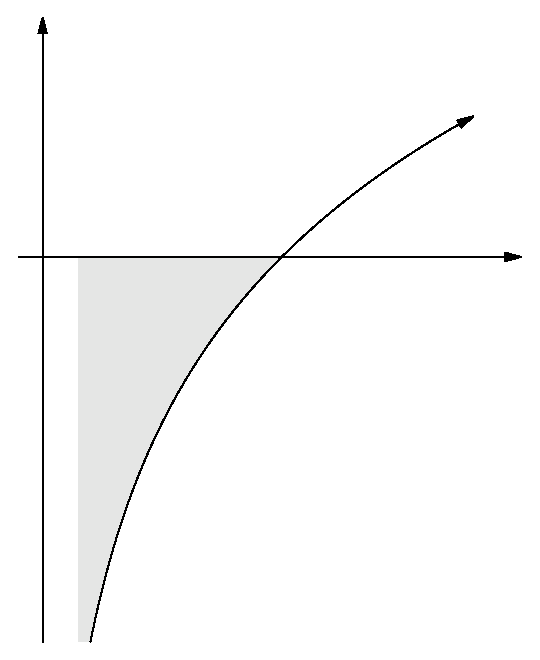
\includegraphics[width=100pt]{ChapterGeom/Figures/ln_3.eps}\\
 & & \\ \hline
 & & \\
0.001 & -0.9921 & \includegraphics[width=100pt]{ChapterGeom/Figures/ln_4.eps}\\
 & & \\ \hline
  & & \\
0.0001 & -0.9989 &\includegraphics[width=100pt]{ChapterGeom/Figures/ln_5.eps} \\
 & & \\ \hline
\end{tabular}
\end{center}
}{0in}

\item As $c$ approaches 0 from the right, what does the area seem to be approaching?

\solushun{It seems to be approaching -1\\}{1in}
\end{itemize}
\end{exercise}

The above calculation motivates the definition of an improper integral.

\FormulaBox{Definition of Improper Integral I}{
\begin{tabular}{c}

If $f(x)$ has a vertical asymptote at $x=a$ \\ but is continuous on the interval $\left(a,b\right]$, \\
then the improper integral is defined as \\ $\int_a^b f(x) \dif x = \lim_{c\rightarrow a^+} \int_c^b f(x) \dif x $

\end{tabular}
}

If this limit converges to a number, then we say the \conv{improper integral} \emph{converges}.  Otherwise, we say the \divergence{improper integral} \emph{diverges}.
 We apply the definition to finish off the above exercise.

\begin{example}{Area Between the Axes and Natural Log}
To calculate the area between $y=0$, $x=0$, and $y=\ln(x)$, we use the definition of improper integral.  We proceed with the following calculation: 
\begin{align*}
\int_0^1 \ln(x) \dif x &= \lim_{c\rightarrow 0^+} \int_c^1 \ln(x) \dif x \\
&=\lim_{c\rightarrow 0^+}  \left. x\ln(x)-x \right]_{x=c}^{x=1} \\
&=\lim_{c\rightarrow 0^+}  \left(1\ln(1)-1\right) -\left(c\ln(c)-c\right)
\end{align*}

In the above limit, all terms are harmless except for $\lim_{c\rightarrow 0}c\ln(c)$, which is indeterminate of the form $0\cdot \infty$.  We can rewrite as $$\lim_{c\rightarrow 0^+}c\ln(c)=\lim_{c\rightarrow 0^+}\frac{\ln(c)}{\left(\frac{1}{c}\right)}$$ to get it in the form $\frac{\infty}{\infty}$ (up to a minus sign which is harmless), where we can apply LHR.
\end{example}

\begin{exercise}{We'll Actually Finish This Problem Here, Promise \Coffeecup \Coffeecup}
Finish evaluating the limit above and verify the area matches your estimations from Exercise \ref{VertUnbounded}.\ref{LogArea}.
\solushun{\begin{align*}
\lim_{c\to0^+}\frac{\ln(c)}{\frac{1}{c}}&=\lim_{c\to0^+}\frac{\frac{1}{c}}{-1\frac{1}{c^2}}\tag{By LHR}\\
&=\lim_{c\to0^+}-c=0
\end{align*}
Then, we can evaluate the original integral:
$$\lim_{c\rightarrow 0^+}  \left(1\ln(1)-1\right) -\left(c\ln(c)-c\right)=(1\cdot0-1)-0=-1$$
}{1in}
\end{exercise}

Let us now construct the analogous definition for a vertical asymptote occurring at the right-hand endpoint rather than the left-hand endpoint.

\begin{exercise}{Completing the Definition \Coffeecup \Coffeecup \Coffeecup}

Suppose a function $f(x)$ is continuous on $[a,b)$ but had a vertical asymptote at $x=b$.  Use the diagram below to help complete the definition of such an improper integral.  Fill in the boxes below.

\FormulaBox{Definition of Improper Integral II}{
\begin{tabular}{c}

If $f(x)$ has a vertical asymptote at $x=a$ \\ but is continuous on the interval $\left(a,b\right]$, \\
then the improper integral is defined as \\ $\int_a^b f(x) \dif x = \lim_{c\rightarrow \square } \int_\square^\square f(x) \dif x $

\end{tabular}
}
\begin{center}
    \includegraphics[width=300pt]{ChapterGeom/Figures/abcint.eps}
\end{center}
Once again, if this limit converges to a number, then we say the \conv{improper integral} \emph{converges}.  Otherwise, we say the \divergence{improper integral} \emph{diverges}.
\end{exercise}

\begin{exercise}{Illustrate the Computation  \Coffeecup} Here we demonstrate an example of computing an improper integral with the vertical asymptote at the right-hand endpoint.  Illustrate the computation on the axes below.  Show the graph of the integrand and the locations of the bounds $a,b,$ and $c$.  

\begin{align*}
\int_{x=0}^{x=\pi/2}\tan(x)\dif x &= \lim_{c\rightarrow \pi/2^-}\int_{x=0}^{x=c}\tan(x)\dif x \\
&=\lim_{c\rightarrow \pi/2^-}\left. -\ln\left(\cos(x)\right)\right]_{x=0}^{x=c} \\
&=\lim_{c\rightarrow \pi/2^-} -\ln\left(\cos\left(c\right)\right)+\ln\left(\cos(0)\right) \\
&=\infty
\end{align*}
\begin{center}
\includegraphics[scale=0.8]{quad1.eps}
\end{center}
\solushun{\begin{center}
\includegraphics[scale=0.8]{ChapterGeom/Figures/tanintsolushun.eps}
\end{center}
}{0in}
\end{exercise}

If the vertical asymptote is in the interior (rather than at an endpoint) of the interval over which you are integrating, it may be necessary to split it into several integrals.

\begin{example}{A Particular Unbounded Region }
Suppose we wish to calculate the area bounded by the $x$-axis, the line $x=1$, the line $x=-1$, and the graph of $f(x)=\frac{1}{\sqrt{|x|}}$.  Notice the function has a vertical asymptote at $x=0$, which is in the interior of the interval over which we wish to integrate.  Thus, we split the integral into two integrals.  The first has a vertical asymptote at the right-hand endpoint and the second has a vertical asymptote at the left-hand endpoint.  We handle each accordingly.

\begin{align*}
\int_{-1}^{1} \frac{1}{\sqrt{|x|}}\dif x&=\int_{-1}^{0} \frac{1}{\sqrt{|x|}}\dif x+\int_{0}^{1} \frac{1}{\sqrt{|x|}}\dif x \\ 
&=\lim_{c_1 \rightarrow 0^-} \int_{-1}^{c_1} \frac{1}{\sqrt{|x|}} \dif x + \lim_{c_2 \rightarrow 0^+} \int_{c_2}^1 \frac{1}{\sqrt{|x|}} \dif x 
\end{align*} 

We now evaluate each of those integrals separately and add their totals.
\begin{align*}
\lim_{c_1 \rightarrow 0^-} \int_{-1}^{c_1} \frac{1}{\sqrt{|x|}} \dif x &=\lim_{c_1 \rightarrow 0^-} \left. {-2\sqrt{|x|}}\right|_{x=-1}^{x=c_1} \\
&=\lim_{c_1 \rightarrow 0^-}  {-2\sqrt{-c_1}}+2\sqrt{1} \\
&=0+2 \\
&=2
\end{align*}
The other region is just a reflection across the $y$-axis and thus must also have area 2. We conclude $$ \int_{-1}^{1} \frac{1}{\sqrt{|x|}}\dif x=4 $$

	\begin{center}       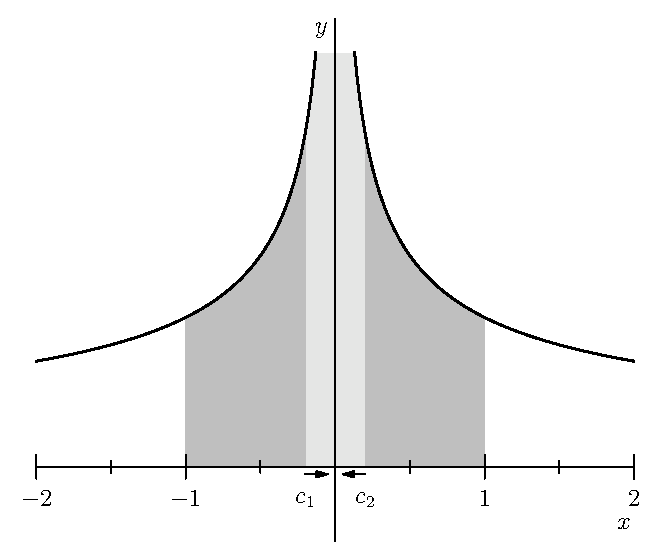
\includegraphics[width=300pt]{ChapterGeom/Figures/onesqrtx.eps}
    \end{center}
 \end{example}
 
\begin{exercise}{Some Subtle Sign Business \Coffeecup}
In the above computation, why is there a negative sign on the antiderivative, producing $-2\sqrt{|x|}$ instead of just $2\sqrt{|x|}$?  ({\bf Hint:} Graph the function $2\sqrt{|x|}$!)
\solushun{In order to evaluate the integral of an absolute value function, we treat it as a piecewise function. So:
$$\int\frac{1}{\sqrt{|x|}}\dif x=\int\frac{1}{\sqrt{-x}}\dif x=\int(-x)^{-\frac{1}{2}}\dif x=-2\sqrt{-x}$$ Since $-x=|x|$ when $x<0$, we can write $-2\sqrt{|x|}$.\\
}{1in}
\end{exercise}

Ok, now you give it a shot!  
\begin{exercise}{Improper Integral Practice \Coffeecup \Coffeecup}
Evaluate the following integrals and draw graphs similar to the figure above.  Show how you are evaluating the improper integral as a limit of integrals of bounded regions.
\begin{itemize}
\item $\int_{2}^4\frac{1}{\sqrt{x-2}}\dif x $

\solushun{\begin{align*}
\int_{2}^4\frac{1}{\sqrt{x-2}}\dif x &=\lim_{c\to2^+}\int_{c}^4\frac{1}{\sqrt{x-2}}\dif x\\
&=\lim_{c\to2^+}\left.2\sqrt{x-2}\right|^4_c\\
&=\lim_{c\to2^+}2\sqrt{2}-2\sqrt{c-2}=2\sqrt{2}
\end{align*}}{2in}

\item $ \int_{2}^4 \frac{1}{x^2-4}\dif x $

\solushun{
\begin{align*}
\int_{2}^4 \frac{1}{x^2-4}\dif x&=\lim_{c\to2^+}\int_{x=c}^{x=4}\frac{1}{x^2-4}\dif x\\
&=\lim_{c\to2^+}\frac{1}{4}\int_{x=c}^{x=4}\frac{1}{x-2}-\frac{1}{x+2}\dif x\tag{Via PFD}\\
&=\lim_{c\to2^+}\frac{1}{4}\left[\ln\left|x-2\right|-\ln\left|x+2\right|\right]^4_c\\
&=\lim_{c\to2^+}\frac{1}{4}\left[\ln\left|\frac{x-2}{x+2}\right|\right]^4_c\\
&=\lim_{c\to2^+}\frac{1}{4}\left[\ln\left|\frac{2}{6}\right|-\ln\left|\frac{c-2}{c+2}\right|\right]\\
&=\lim_{c\to2^+}\frac{1}{4}\left[\ln\left|\frac{2}{6}\right|-(-\infty)\right]=\infty\\
\end{align*}}{2in}

\item $ \int_{0}^{\pi /2} \sec(x) \dif x $
\solushun{
\begin{align*}
\int_{0}^{\pi /2} \sec(x) \dif x &=\lim_{c\to\frac{\pi}{2}^-}\int_{0}^{c} \sec(x) \dif x\\
&=\lim_{c\to\frac{\pi}{2}^-}\ln\left|\sec(x)+\tan(x)\right|^c_0\\
&=\lim_{c\to\frac{\pi}{2}^-}\ln\left|\sec(c)+\tan(c)\right|-\ln\left|\sec(0)+\tan(0)\right|\\
&=\ln\left|\infty+\infty\right|-\ln\left|1\right|=\infty\\
\end{align*}}{2in}
\item $ \int_{-\pi/2}^{\pi /2} \csc^2(x) \dif x $

\solushun{
\begin{align*}
\int_{-\pi/2}^{\pi /2} \csc^2(x) \dif x&=\lim_{c_1\to0^-}\int_{-\pi/2}^{c_1} \csc^2(x) \dif x+\lim_{c_2\to0^+}\int_{c_2}^{\pi/2} \csc^2(x) \dif x
\end{align*}
Since the function is symmetric, we can start with just the left side.
\begin{align*}
\lim_{c\to0^-}\int_{-\pi/2}^{c} \csc^2(x) \dif x&=\lim_{c\to0^-}\left[\cot(x)\right]^c_{-\pi/2}\\
&=\lim_{c\to0^-}\cot(c)-\cot(-\pi/2)=\infty-0=\infty\\
\end{align*}
Since the function is symmetric, we can double the result, which is the same.}{2in}

\end{itemize}
\AnswerKeyEntry{The integrals evaluate to $2\sqrt{2},\infty,\infty,$ and $\infty$.}
\end{exercise}

\subsection{Horizontally Unbounded Regions}

If the integral is over an interval that includes plus or minus infinity as one of the endpoints, we must proceed by approximating via a bounded interval and then taking the limit as the endpoint goes to plus or minus infinity.

\FormulaBox{Definition of Improper Integral III}{\begin{tabular}{c}
Let $f(x)$ be continuous on the interval $\left[a,\infty\right)$ for some real number $a$. \\ Then we define
$ \int_{a}^\infty f(x)\dif x = \lim_{c \rightarrow \infty} \int_{a}^c f(x)\dif x. $ 
\end{tabular}}
An integral to negative infinity is defined analogously via the corresponding limit. 

\begin{exercise}{Finding $c$ \Coffeecup}
	\begin{center}
        \includegraphics[width=300pt]{ChapterGeom/Figures/unboundhorizont.eps}
	\end{center}
Here is a graph that represents the above definition for $a=0$.  Interpret the definition by labeling $c$ on the graph and explaining the role it plays.  
    \solushun{
        \begin{center}
            \includegraphics[width=300pt]{ChapterGeom/Figures/unboundedhorizonSoln_cropped-eps-converted-to.pdf}
        \end{center}
        Here $c$ is the upper bound of integration, and by taking it in the limit, we are looking at the behavior of the integral as its upper bound increases.\\
    }{1in}
\end{exercise}

\begin{example}{Area Under $f(x)=\frac{1}{x^2}$}

	\begin{wrapfigure}{r}{0.3\textwidth}
    	\centering
		\includegraphics[width=0.3\textwidth]{ChapterGeom/Figures/AreaUnder1Overx2}
	\end{wrapfigure}

Suppose we wish to compute the area under the curve $f(x)=\frac{1}{x^2}$ over the interval $\left[1,\infty\right)$.  We apply the definition of the improper integral as a limit of bounded integrals.  

\begin{align*}
\int_{x=1}^{x=\infty}\frac{1}{x^2}\dif x &= \lim_{c \rightarrow \infty} \int_{x=1}^{x=c} \frac{1}{x^2} \dif x \\
&= \lim_{c \rightarrow \infty} \left.-\frac{1}{x} \right]_{x=1}^{x=c}\\
&= \lim_{c \rightarrow \infty} -\frac{1}{c}+\frac{1}{1} \\
&=1
\end{align*}
Thus, the area under the curve is 1.
\end{example}

\begin{exercise}{Area Under $1/x^p$ \Coffeecup \Coffeecup \Coffeecup}
\begin{itemize}
\item Calculate the improper integral $\int_{x=1}^{x=\infty}\frac{1}{x^3}\dif x$.

\solushun{
\begin{align*}
\int_{x=1}^{x=\infty}\frac{1}{x^3}\dif x&=\lim_{c\to\infty}\int_{x=1}^{x=c}\frac{1}{x^3}\dif x\\
&=\lim_{c\to\infty}\left.-\frac{1}{2x^2}\right|_{x=1}^{x=c}\\
&=\lim_{c\to\infty}-\frac{1}{2c^2}+\frac{1}{2(1)^2}=\frac{1}{2}
\end{align*}
}{1in}

\item Calculate the improper integral $\int_{x=1}^{x=\infty}\frac{1}{x^{1}}\dif x$.

\solushun{
\begin{align*}
\int_{x=1}^{x=\infty}\frac{1}{x^{1}}\dif x&=\lim_{c\to\infty}\int_{x=1}^{x=c}\frac{1}{x^{1}}\dif x\\
&=\lim_{c\to\infty}\ln(x)|^{x=c}_{x=1}\\
&=\lim_{c\to\infty}\ln(c)-\ln(1)=\infty-0=\infty
\end{align*}}{1in}

\item Calculate the improper integral $\int_{x=1}^{x=\infty}\frac{1}{x^{1/2}}\dif x$.
\solushun{
\begin{align*}
\int_{x=1}^{x=\infty}\frac{1}{x^{1/2}}\dif x&=\lim_{c\to\infty}\int_{x=1}^{x=c}\frac{1}{x^{1/2}}\dif x\\
&=\lim_{c\to\infty}\left.2x^{\frac{1}{2}}\right|_{x=1}^{x=c}\\
&=\lim_{c\to\infty}2c^{\frac{1}{2}}-2(1)^{\frac{1}{2}}\\
&=\infty-2=\infty
\end{align*}}{1in}
\item For what real numbers $p$ will $\int_{x=1}^{x=\infty}\frac{1}{x^{p}}\dif x$ converge?  For what $p$ will it diverge?
\solushun{For $p>1$, the $\int_{x=1}^{x=\infty}\frac{1}{x^{p}}\dif x$ will converge because the antiderivative of $x^{-p}, p>1$ will not transform the function into one with positive growth order (a positive exponent). However, the antiderivative of any function $x^{-p}, p\leq1$ will have a positive exponent and thus will diverge.\\}{1in}
\end{itemize}
\end{exercise}

If the integral is across the entire real number line, one must split into two separate integrals, similar to how we handled a vertical asymptote in the interior of our interval.  


\FormulaBox{Definition of Improper Integral III}{\begin{tabular}{c}
Let $f(x)$ be continuous on the entire real number line. \\ For any real number $a$, we define 
$ \int_{-\infty}^\infty f(x)\dif x = \int_{-\infty}^a f(x)\dif x + \int_{a}^\infty f(x)\dif x.$ 
\end{tabular}}

For the following problems, you may spot yourself the following fact we will prove in Calc 3: $$ \int_{-\infty}^\infty e^{-x^2}\dif x = \sqrt{\pi}$$

\begin{exercise}{More Practice with Improper Integrals \Coffeecup \Coffeecup}

Now, try the following integrals and for each draw a graph like the above figure that represents your integral as a limit of integrals of bounded regions.  Also, for the following problems, you may spot yourself the following fact we will prove in Calc 3: $$ \int_{-\infty}^\infty e^{-x^2}\dif x = \sqrt{\pi}$$


\begin{itemize}
\item $ \int_{0}^\infty xe^{-x^2}\dif x $
\solushun{
Via u-sub, let $u=-x^2, \dif u=-2x\dif x$.
\begin{align*}
\int_{0}^\infty xe^{-x^2}\dif x&=\lim_{c\to\infty}-\frac{1}{2}\int_{0}^c e^{u}\dif\\
&=\lim_{c\to\infty}-\frac{1}{2}\int_{0}^c e^{u}\dif\\
&=\lim_{c\to\infty}-\frac{1}{2}\left.e^{-x^2}\right|^c_0\\
&=\lim_{c\to\infty}-\frac{1}{2}\cdot\left[e^{-c^2}-e^0\right]\\
&=\frac{1}{2}
\end{align*}}{1.5in}

\item $ \int_{-\infty}^\infty xe^{-x^2}\dif x $
\solushun{\begin{align*}
\int_{-\infty}^\infty xe^{-x^2}\dif x&=\lim_{c_1\to-\infty}-\frac{1}{2}\int_{c_1}^0 e^{u}\dif+\lim_{c_2\to\infty}-\frac{1}{2}\int_{0}^{c_2} e^{u}\dif\\
&=\lim_{c_1\to\infty}-\frac{1}{2}\cdot\left[e^{-x^2}\right]_{c_1}^0+\lim_{c_2\to\infty}-\frac{1}{2}\cdot\left[e^{-x^2}\right]_{0}^{c_2}\\
&=\lim_{c_1\to\infty}-\frac{1}{2}\cdot\left[1-e^{-c_1^2}\right]+\lim_{c_2\to\infty}-\frac{1}{2}\cdot\left[e^{-c_2^2}-1\right]\\
&=-\frac{1}{2}+\frac{1}{2}=0
\end{align*}
Then we need to add on the other half of the function. It's always positive so we can just double the value to get $\frac{1}{2}\sqrt{\pi}$\\}{1.5in}

\item $ \int_{-\infty}^\infty x^2 e^{-x^2}\dif x $
\solushun{$$\int_{-\infty}^\infty x^2e^{-x^2}\dif x=\lim_{c_1\to-\infty} \int_{c_1}^0 x^2e^{-x^2}\dif x + \lim_{c_2\to\infty} \int_{0}^{c_2} x^2e^{-x^2}\dif x\\
$$
Since the function is symmetrical, we can deal with just the first half of the sum. Via IBP, let $u=x, \dif u = \dif x, v=-\frac{1}{2}e^{-x^2}, \dif v = xe^{-x^2}$ (we are leveraging what we did in the last problem):
\begin{align*}
\lim_{c_1\to-\infty} \int_{c_1}^0 x^2e^{-x^2}\dif x&=\lim_{c_1\to-\infty}\left.-\frac{1}{2}xe^{-x^2}\right|^{0}_{c_1}+\frac{1}{2}\int^0_{c_1} e^{-x^2}\dif x\\
&=\lim_{c_1\to-\infty} c_1e^{-c_1^2} +\frac{1}{4}\sqrt{\pi}\\
&=\lim_{c_1\to-\infty} \frac{c_1}{e^{c_1^2}}+\frac{1}{4}\sqrt{\pi}\\
&=\lim_{c_1\to-\infty} \frac{1}{e^{c_1^2}}+\frac{1}{4}\sqrt{\pi}\tag{By LHR}\\
&=\frac{1}{4}\sqrt{\pi}
\end{align*}
Adding on the other half gives $\frac{\sqrt{\pi}}{2}$\\}{1.5in}
\item $ \int_{2}^\infty \frac{1}{x\ln(x)}\dif x $
\solushun{\begin{align*}
\int_{2}^\infty \frac{1}{x\ln(x)}\dif x &=\lim_{c\to\infty}\int^c_2\frac{1}{x\ln(x)}\dif x\\
&=\lim_{c\to\infty}\int^c_2\frac{1}{u}\dif u\\
&=\lim_{c\to\infty}\left.\ln(u)\right|^c_2\\
&=\lim_{c\to\infty}\left.\ln(\ln(x))\right|^c_2\\
&=\lim_{c\to\infty}\ln(\ln(c))-\ln(\ln(2))\\
&=\infty-2=\infty
\end{align*}}{1.5in}
\item $ \int_{2}^\infty \frac{1}{x(\ln(x))^2}\dif x $
\solushun{\begin{align*}
\int_{2}^\infty \frac{1}{x(\ln(x))^2}\dif x &=\lim_{c\to\infty}\int^c_2\frac{1}{x(\ln(x))^2}\dif x\\
&=\lim_{c\to\infty}\int^c_2\frac{1}{u^2}\dif u\\
&=\lim_{c\to\infty}\left.-\frac{1}{u}\right|^c_2\\
&=\lim_{c\to\infty}\left.-\frac{1}{\ln(x)}\right|^c_2\\
&=\lim_{c\to\infty}-\frac{1}{\ln(c)}+\frac{1}{\ln(2)}\\
&=\frac{1}{\ln(2)}
\end{align*}
}{1.5in}
\item Consider the integral $\int_0^{\infty} \sin(x) \dif x $.  Explain why it would be incorrect to say that all the positive and negative area cancel each other out to be zero. In particular, cite the definition of the improper integral as a limit in your explanation. 
\solushun{An improper integral is defined using a limit, and here the limit does not exist, as the area keeps going up and down by the same amount forever.}{1in}
\end{itemize}
\AnswerKeyEntry{\textbullet The area under $xe^{-x^2}$ from zero to $\infty$ is $\frac{1}{2}$. \textbullet Splitting into two integrals at $x=0$ produces one of area one-half and one of area negative one-half, so the total integral is zero. 
\textbullet After applying IBP with $u=x$ and $\dif v = xe^{-x^2}\dif x$, one obtains $\frac{\sqrt{\pi}}{2}$ as the area under the curve.
\textbullet The area under $\frac{1}{x\ln(x)}$ from 2 to $\infty$ is infinite. \textbullet The area under $\frac{1}{x\left(\ln(x)\right)^2}$ from 2 to $\infty$ is $\frac{1}{\ln(2)}$. 
\textbullet An improper integral is defined using a limit, and here the limit does not exist, as the area keeps going up and down by the same amount forever.}
\end{exercise}
